Algoritmos como K-Means presentan dificultades para identificar clusters cuando las distancias entre elementos de un mismo conjunto es mayor que la de elementos de conjuntos distintos.
En estos casos, puesto que K-Means busca minimizar la distancia entre los elementos dentro de un mismo cluster, producirá clusters que difieran significativamente de los grupos <<correctos>>.
Podemos observar un ejemplo en el escenario de la figura~\ref{img:kmeans-dbscan}, donde se compara el resultado de K-Means con el del algoritmo que analizamos en esta sección, conocido como \textit{DBSCAN}.

\begin{figure}[!h]
    \centering
    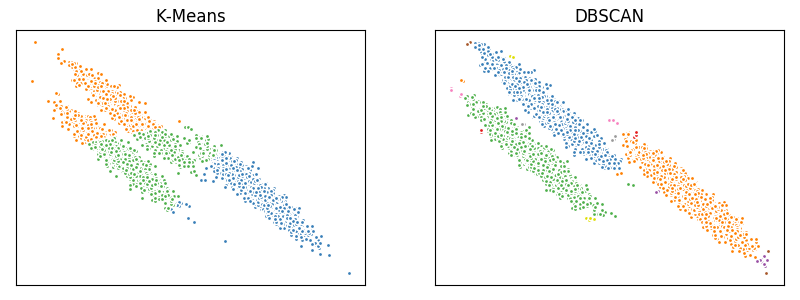
\includegraphics[width=\textwidth]{kmeans-dbscan.png}
    \caption{Resultados de los algoritmos K-Means y DBSCAN ejecutados sobre un conjunto de datos que sigue una distribución anisotrópica.}
    \label{img:kmeans-dbscan}
\end{figure}

En la imagen podemos observar asimismo el comportamiento de otro algoritmo sobre el mismo conjunto de datos.
En esta sección abordamos el algoritmo en cuestión, denominado \textit{DBSCAN}~\footnote{Siglas en inglés de \textit{Density-based spatial clustering of applications with noise}.}, que forma parte del conjunto de algoritmos de clustering basados en la densidad de los datos.

Un cluster basado en el criterio de densidad de los puntos consiste en un área densa de puntos conectados, separado de otros clusters por áreas de menor densidad.

\subsection{Densidad}\label{subsec:densidad}

El algoritmo DBSCAN define la densidad alrededor de un punto como la cantidad de puntos localizados alrededor de este en un radio, $Eps$, específico.
El propio punto es incluido en este conteo.
En la figura~\ref{img:dbscan} se puede observar gráficamente esta definición.
En este caso número de puntos alrededor de $A$ es 7.

El valor del radio es determinante en la densidad de un punto.
Si este valor es suficientemente grande, entonces todos los puntos tendrán una densidad de $n$, el número de puntos en el conjunto de datos.
En cambio, si el radio es demasiado pequeño, la densidad de todos los puntos será igual a 1.
Más adelante discutiremos algunas estrategias para la selección de valores apropiados para el radio.

\begin{figure}[!h]
    \centering
    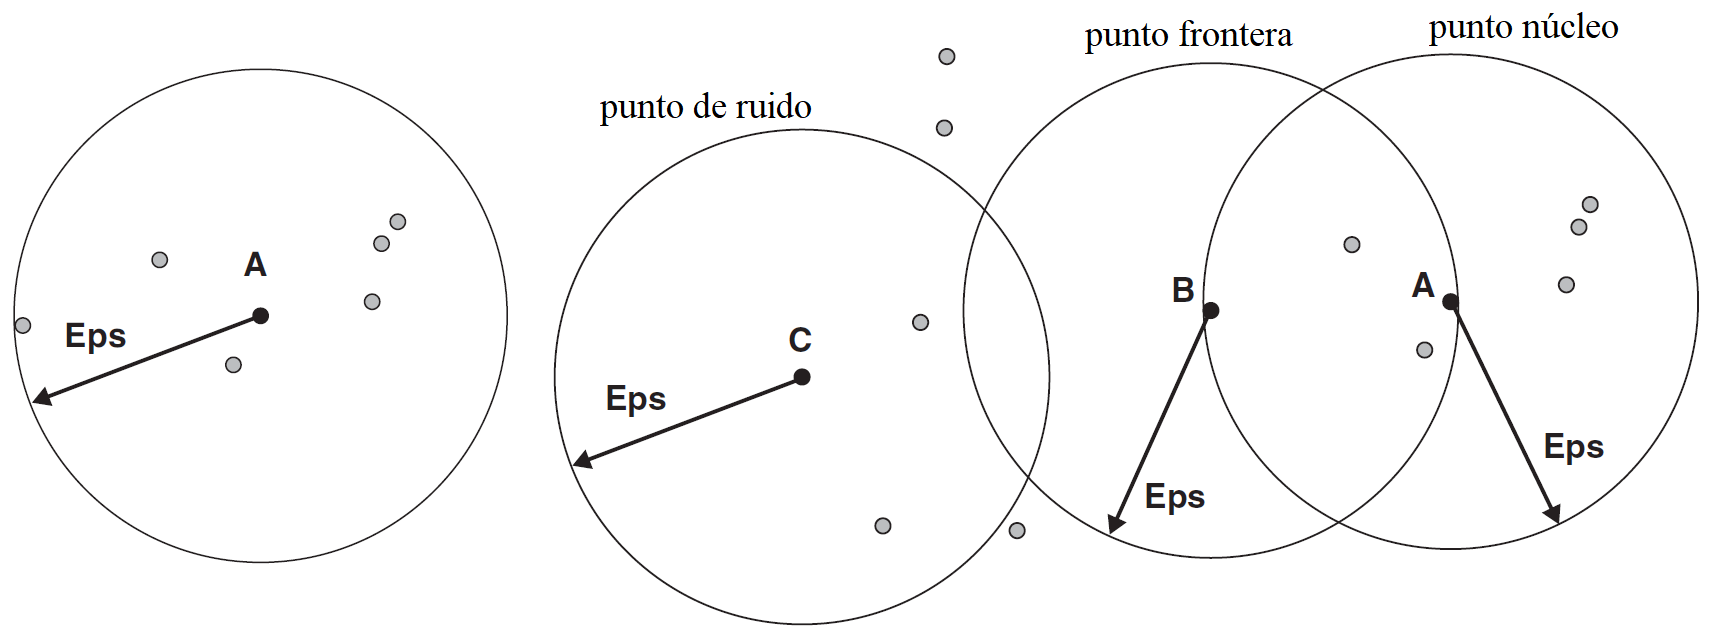
\includegraphics[width=\textwidth]{dbscan.png}
    \caption{Densidad en el entorno de un punto y clasificaciones de los puntos según su densidad. (Tomado de~\cite{Tan05}.)}
    \label{img:dbscan}
\end{figure}

De acuerdo con la densidad de un punto, estos pueden ser clasificados de la siguiente forma:

\begin{itemize}
    \item \textbf{Puntos núcleo}: Constituyen puntos de la región interna de un cluster basado en densidad.
    Un punto es núcleo si el número de puntos alrededor de este (incluyéndolo) supera o iguala un valor $MinPts$, especificado por el usuario.
    En la figura~\ref{img:dbscan} los puntos identificados con la letra $A$ son núcleos para el radio $Eps$ indicado si $MinPts\leq 7$.
    \item \textbf{Puntos frontera}: Un punto frontera es aquel que no cumple el criterio de núcleo, pero que forma parte de la vecindad de al menos uno de estos.
    En la figura~\ref{img:dbscan} $B$ es un punto frontera.
    \item \textbf{Puntos de ruido}: Un punto es de ruido si no es núcleo o frontera.
    En la figura~\ref{img:dbscan} $C$ es un punto de ruido.
\end{itemize}

\subsection{Algoritmo DBSCAN}\label{subsec:algoritmoDbscan}

A partir de las definiciones dadas de puntos núcleos, fronteras y de ruido, podemos describir el algoritmo DBSCAN del siguiente modo: Todo par de puntos núcleos cuya distancia sea no mayor que $Eps$ son asignados al mismo cluster.
De igual forma, los puntos fronteras son asignados al cluster de los puntos núcleos cuya distancia a estos sea menor o igual que $Eps$.
(En caso de estar en la vecindad de núcleos pertenecientes a clusters diferentes, un criterio específico debe ser determinado al programar el algoritmo).
Los puntos de ruido son descartados y no asignados a ningún cluster.

\begin{algorithm}
    \caption{DBSCAN}
    \label{algorithm:DBSCAN}
    Etiquetar todos los puntos como núcleo, frontera o ruido\;
    Eliminar los puntos de ruido\;
    Añadir una arista entre todo par de puntos núcleos que se encuentren a una distancia menor o igual que $Eps$\;
    Convertir cada componente conexa del grafo resultante en un cluster\;
    Asignar cada punto frontera a uno de los clusters de los puntos núcleos asociados a este\;
\end{algorithm}

\subsubsection{Complejidad espacial y temporal}

El algoritmo DBSCAN demora en ejecución un tiempo $O(n \cdot$ tiempo para encontrar puntos en una $Eps$-vecindad), donde $n$ es el número de puntos en el conjunto de datos.
En el peor caso, esta complejidad sería $O(n^2)$.
Sin embargo, el uso de determinadas estructuras de datos en espacios de pocas dimensiones, permite la recuperación eficiente de todos los puntos en un intervalo dado alrededor de un punto específico~\cite{Tan05};
en estos escenarios la complejidad puede llegar a ser $O(n\log n)$.
Los requerimientos de memoria de DBSCAN, aun en espacios de grandes dimensiones, son $O(n)$, puesto que solo es necesario mantener poca información relativa a cada punto, como puede ser el cluster al que pertenece, la clasificación, etc.
No obstante, este uso de memoria depende igualmente del comportamiento de la estructura de datos empleada para computar las vecindades.

\subsubsection{Selección de parámetros para DBSCAN}

Un criterio para determinar los parámetros es mediante la observación del comportamiento de la distancia de los puntos a su $k$-ésimo vecino más cercano, conocida como $k$-distancia.
Si un punto pertenece a un cluster, entonces su $k$-distancia debe ser un valor relativamente pequeño, siempre que $k$ no sea mayor que el tamaño del cluster.
Siempre que las densidades de los clusters no difieran radicalmente, en promedio, los valores de la $k$-distancias para puntos que pertenezcan a algún cluster no mostrarán un rango de valores muy amplio.
En cambio, para puntos que no pertenezcan a ningún cluster, es decir, de ruido, este valor sí estará situado muy por encima del rango antes mencionado.
De esta forma, si tomamos todos los puntos de un conjunto de datos, los ordenamos por su $k$-distancia y estas las representamos en una gráfica, deberíamos obtener una imagen donde existirá un punto de inflexión que se corresponda con el valor de la $k$-distancia a partir del cual los puntos se encuentran fuera de algún cluster.
Podemos entonces tomar dicho valor como el $Eps$ adecuado para el problema en cuestión.
En cuanto al valor de $MinPts$, este sería precisamente el $k$ seleccionado para calcular las distancias, pues los puntos cuya $k$-distancia sea menor que $Eps$ serán etiquetados como núcleos, mientras los demás serán fronteras o ruido.

% TODO Consider putting an example of graphic here

Es importante notar que el valor de $Eps$ resultante de este proceso dependerá del $k$ seleccionado al inicio.
Si $k$ es demasiado pequeño, algunos puntos de ruido situados muy próximos entre sí pudieran ser etiquetados incorrectamente como clusters.
Por otra parte, si $k$ es demasiado grandes, aquellos clusters cuya cantidad de elementos sea menor que $k$ no serán identificados correctamente.

Un defecto del algoritmo DBSCAN es que requiere que las densidades de los clusters (y del espacio de datos en general) muestren comportamientos semejantes.
Un ejemplo de esta afirmación podemos observarlo en la figura~\ref{img:density-issues}.
El ruido alrededor de los clusters $A$ y $B$ presenta la misma densidad que los clusters $C$ y $D$.
Si seleccionamos un $Eps$ suficientemente bajo para detectar a $C$ y $D$, sucederá entonces que $A$, $B$ y el ruido a su alrededor constituirán un mismo cluster.
En cambio si el $Eps$ es tan alto como para distinguir a $A$ y $B$ como clusters independientes, entonces los puntos que forman parte de $C$ y $D$ serán considerados ruido.

\begin{figure}[!h]
    \centering
    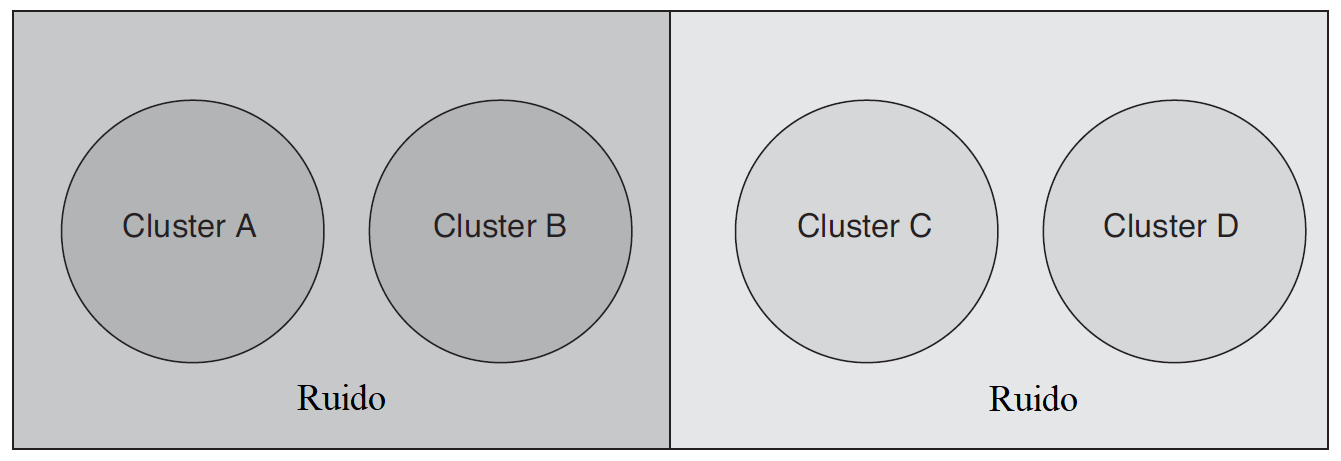
\includegraphics[width=\textwidth]{density-issues.png}
    \caption{Cuatro clusters en un entorno de ruido.
    Los tonos de gris más oscuros indican mayores densidades. (Tomado de~\cite{Tan05}.)}
    \label{img:density-issues}
\end{figure}

% TODO Consider adding HDBSCAN